\section{Simulation case: reconstruction of known physical jerk}
\label{sec:synthetic-case}

\subsection{What was simulated and what was held fixed}
The known-truth simulation contains $1{,}296$ frozen
confirmatory trajectories from the six prespecified
vehicle jerk regimes: zero jerk, positive and negative
constant jerk, sinusoidal jerk, abrupt jerk reversal and
a finite braking-related jerk pulse. At each of three
position-noise levels ($0.03$, $0.12$, $0.30$\,m)
we consider independent observation errors,
serially correlated errors, and terminal
contamination. Every trial supplies 80 noisy historical
positions, the original clean position and its known
discrete third-difference jerk, and 20 clean future
positions. The pilot and confirmation use distinct
random seeds; the confirmation trajectories
are precisely the original Experiment005 data,
\emph{not} regenerated for the comparisons below.

Experiment006 examined the choice of the reference mean
and smoothing penalty on this data. Its global cubic
OLS reference with continuous profile Gaussian
likelihood attained $2.441$\,m/s$^3$ historical
discrete-jerk RMSE; the corresponding fixed-zero
reference attained $2.587$\,m/s$^3$, while joint
unknown-mean REML attained $3.295$\,m/s$^3$.
The latter result is not paradoxical: maximum
restricted likelihood is not an oracle minimizer
of physical-jerk reconstruction loss.

\subsection{Soft PLS versus hard SVD truncation and conventional smoothers}
We now compare PLS against the \emph{different estimators}
in Eqs.~\eqref{eq:pls-filter}--\eqref{eq:tsvd-filter},
alongside GCV cubic smoothing splines and a
21-point degree-three Savitzky--Golay filter.
For PLS, the $\widehat\mu$ and continuous
profile-likelihood $\lambda$ are read \emph{unchanged}
from the successful Experiment006 archive.
The truncated-SVD methods use this same
training-only cubic reference mean:
one truncation rank is selected from training data
using GCV, and the other is matched to the PLS
effective degrees of freedom. The matched-rank
method is an \emph{ablation} of soft versus hard
spectral shrinkage, not a separate statistically
optimal rank estimate.

\begin{table*}[t]
\centering
\caption{Same 1,296 frozen simulated trajectories: accuracy
against known discrete jerk in the 80-point historical
window, and future \emph{clean} position RMSE averaged
over the first ten future frames (through one second). The future-position comparison uses the
same last-25-point quadratic continuation for
all fitted trends. True jerk is scored with the same
third-difference operator $D_3/(\Delta t)^3$ applied
to the clean positions. Smaller values are preferable;
the columns describe \emph{different physical targets}.}
\label{tab:sim-svd-comparison}
\begin{tabular}{lcc}
\toprule
Historical trend estimator & Jerk RMSE (m/s$^3$)
 & First-1-s position RMSE (m)\\
\midrule
PLS, cubic OLS $\widehat\mu$ + profile ML
& \textbf{2.4413} & \textbf{0.4353}\\
SVD truncation, matched effective complexity
& 2.9416 & 0.4502\\
SVD truncation, training-only GCV rank
& 250.7181 & 0.4889\\
Natural cubic smoothing spline, training GCV
& 60.9131 & 0.4614\\
Savitzky--Golay, 21-point cubic fit
& 36.8291 & 0.4825\\
\bottomrule
\end{tabular}
\end{table*}

\begin{figure*}[t]
\centering
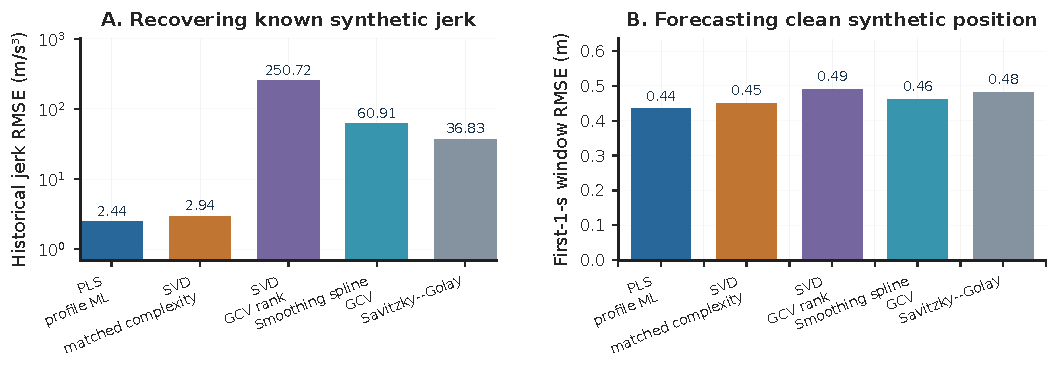
\includegraphics[width=\textwidth]{figures/exp008_known_jerk_benchmarks.pdf}
\caption{Known-truth reconstruction and clean-future forecasting
from the same archived $1{,}296$ simulated trajectories.
(A) Historical third-difference jerk RMSE on a logarithmic
vertical scale (m/s$^3$); (B) clean-position RMSE across the first ten
future frames under the shared 25-point continuation (m).
Truncated SVD is a hard spectral-filtering
\emph{estimator}, not a different implementation
of the PLS linear solve. The GCV-selected
truncation can retain high-frequency components
that strongly amplify differentiation errors.
Different plot axes and units must not be interpreted
as a single aggregate score.}
\label{fig:sim-svd}
\end{figure*}

The matched-complexity comparison isolates an
advantage of soft PLS shrinkage over a hard
roughness-spectral cutoff in the tested
synthetic jerk-reconstruction task.
By contrast, SVD rank chosen to fit observed
positions through GCV is extremely unstable
for \emph{third-difference jerk}:
its historical jerk RMSE is $250.718$\,m/s$^3$,
although its first-second clean-position window
RMSE ($0.489$\,m) is not comparably disastrous.
This distinction is evidence that accurate
position reconstruction and accurate \emph{higher-order
differentiation} are different objectives. The archived
per-trajectory rows identify a concentrated failure:
TSVD-GCV selected rank 75 or 76 of the 77
positive singular directions in 145 of 1,296
trajectories (11.2\%). These cases contributed
78.9\% of that estimator's aggregate squared
historical jerk error. This is an accounting of
the \emph{existing} Experiment008 outcomes,
not a new independent experiment or a separate
selection of particularly favorable trajectories.
Moreover, its rank criterion conditions on the
training-estimated cubic reference $\widehat\mu$,
as explained in Section~\ref{sec:method};
the label ``TSVD-GCV'' denotes that specific
conditional plug-in score, not exact GCV
for the fully data-dependent procedure.

The GCV cubic spline and Savitzky--Golay
comparators likewise smooth positions,
but their respective penalties and local
window mechanisms do not directly impose
the PLS reference constraint
$D_3\tau\approx\mu\mathbf1$. The experiment
does \emph{not} establish that every spline,
window, or SVD denoising procedure is
inferior to PLS; only these prespecified
training-based configurations were evaluated.

\begin{figure*}[t]
\centering
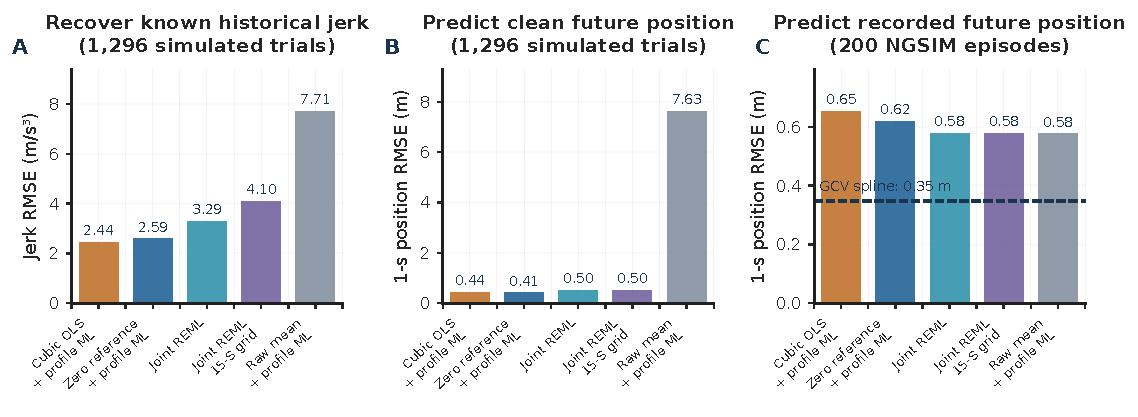
\includegraphics[width=\textwidth]{figures/exp006_reconstruction_forecasting.pdf}
\caption{Additional preexisting Experiment006
reference-mean and parameter-selection comparison.
(A) Historical known-discrete-jerk RMSE in m/s$^3$;
(B) first-second clean-future position-window RMSE in the
same synthetic trajectories; and (C) separately
recorded future-position RMSE from 200 real NGSIM
episodes, with the spline benchmark shown for
context. The different targets, data generating
processes and selected forecast rules explain why
the apparent best method depends on the question.
No real jerk ground truth exists in (C).}
\label{fig:sim-objectives}
\end{figure*}

We therefore distinguish the established
\emph{smoothness-index interpretation} from
the empirical quality of estimated derivatives,
and neither from the separate extrapolation rule.
The calibration experiment in
Section~\ref{sec:precision} is deliberately
reproduced on a different factorial design
with separate known observation-noise and
jerk-innovation interventions; the two
simulation studies must not be pooled as
if they shared one sampling model.
